\iffalse
\documentclass[journal,12pt,twocolumn]{IEEEtran}
\usepackage{amsmath,amssymb,amsfonts,amsthm}
\usepackage{txfonts}
\usepackage{tkz-euclide}
\usepackage{listings}
\usepackage{gvv}
\usepackage[latin1]{inputenc}
\usepackage{array}
\usepackage{pgf}
\usepackage{lmodern}
\usepackage{amsmath}
\begin{document}
\bibliographystyle{IEEEtran}

\title{GATE 2022[EE]-19}
\author{EE23BTECH11066 - Yakkala Amarnath Karthik}
\maketitle
\bibliographystyle{IEEEtran}

\textbf{Question:}\\ \\
The open loop transfer function of a unity gain negative feedback system is given by $G\brak{s}= \frac{k}{s^2 +4s-5}$. The range of k for which the system is stable,is\hfill(GATE EE 2022)\\ \\

\textbf{Solution:}\\ 
\fi
\begin{table}[ht]
  \begin{tabular}{|c|c|c|}
    \hline
    \textbf{Variable} & \textbf{Description} & \textbf{value}\\
    \hline
    $G\brak{s}$ & Open loop transfer function & $\frac{k}{s^2 +4s-5}$\\
   \hline
    1+G$\brak{s}$ & Characteristic equation & 0 \\
    \hline
    \end{tabular}
  \caption{A Table with input parameters}
  \label{tab:gate2022ee19}
\end{table}
\\
 from Table\ref{tab:gate2022ee19}\\
Characteristic equation:
\begin{align}
    1+G\brak{s}=0\\
    \implies 1+\frac{k}{s^2 +4s-5}=0\\
    \implies s^2+4s+\brak{k-5}=0
\end{align}
By routh table analysis, for a stable system:

\begin{center}
    \begin{tabular}{c|c c}
        $s^2$ & 1 & \(k-5\) \\
        $s^1$ & 4 & 0 \\
        $s^0$ & \(\frac{4\brak{k-5}-0}{4}\) & 0 \\
    \end{tabular}
\end{center}


\begin{align}
\frac{4\brak{k-5}-0}{4}>0\\
    k-5>0\\
    \implies k>5
\end{align}

\begin{figure}[ht]
    \centering
    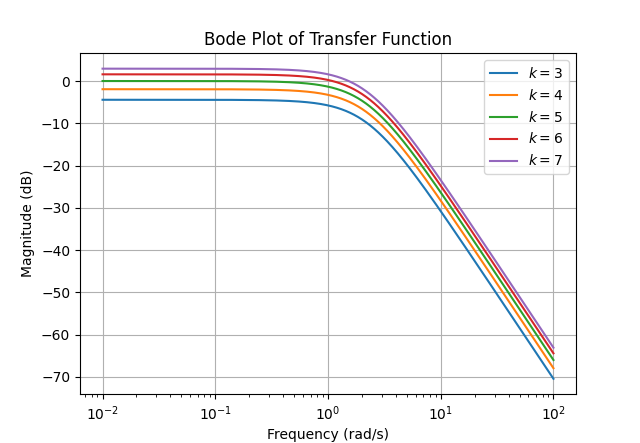
\includegraphics[width=0.45\textwidth]{2022/EE/19/figs/bodeplot.png}
    \caption{Graph showing $k<5,k=5,k>5$}
\end{figure}
For an open transfer function to be stable, its magnitude in the bode plot should be positive for some positive frequency.\\
In the below graph we can observe that the above condition satisfies for k$>$5. 
%\end{document}
